\documentclass[mathserif]{beamer}
\usepackage{amsmath}


\title{An Analysis on Public Health Data\\ of Chronic Kidney Disease}
\author{Akshay Sanjeev }
\date{\today}

\begin{document}

\begin{frame}
    \maketitle
\end{frame}

\begin{frame}
    \tableofcontents
\end{frame}

\section{Preprocessing}
\begin{frame}{Pre-processing}

\end{frame}


\section{Decision Tree}
\begin{frame}{Informal Description}
    \begin{align}
        H^i &= -\sum_j^n p(x^i_j)\log p(x^i_j)\\
        IG^i &= H^i - \sum_s \frac{|x^{is}|}{|x^{i}|} H^is
    \end{align}
    \[x_{\text{selected}} = \arg \max_{i} (IG^i)\]
\end{frame}

\begin{frame}{Results}
    \begin{figure}
        \centering
        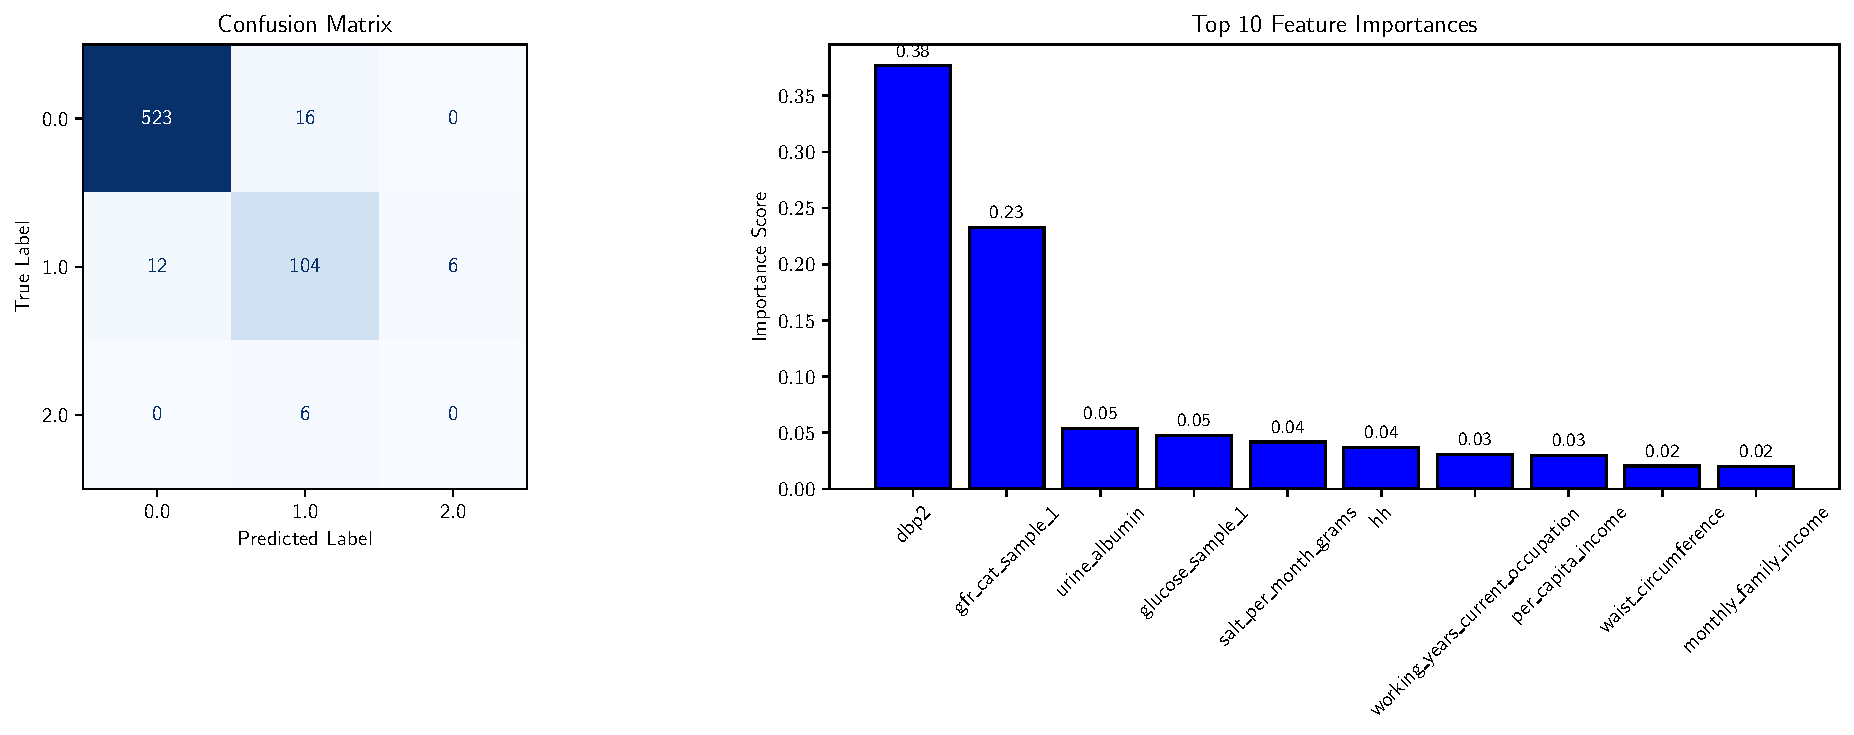
\includegraphics[scale=.35]{DT_summary.pdf}
    \end{figure}
\end{frame}


\section{Random Forest}
\begin{frame}{Informal Description}
    \[\hat{f}_{\text{avg}}(x) = \frac{1}{B}\sum_{i=1}^B \hat{f}^i(x)\]
\end{frame}

\begin{frame}{Results}
    \begin{figure}
        \centering
        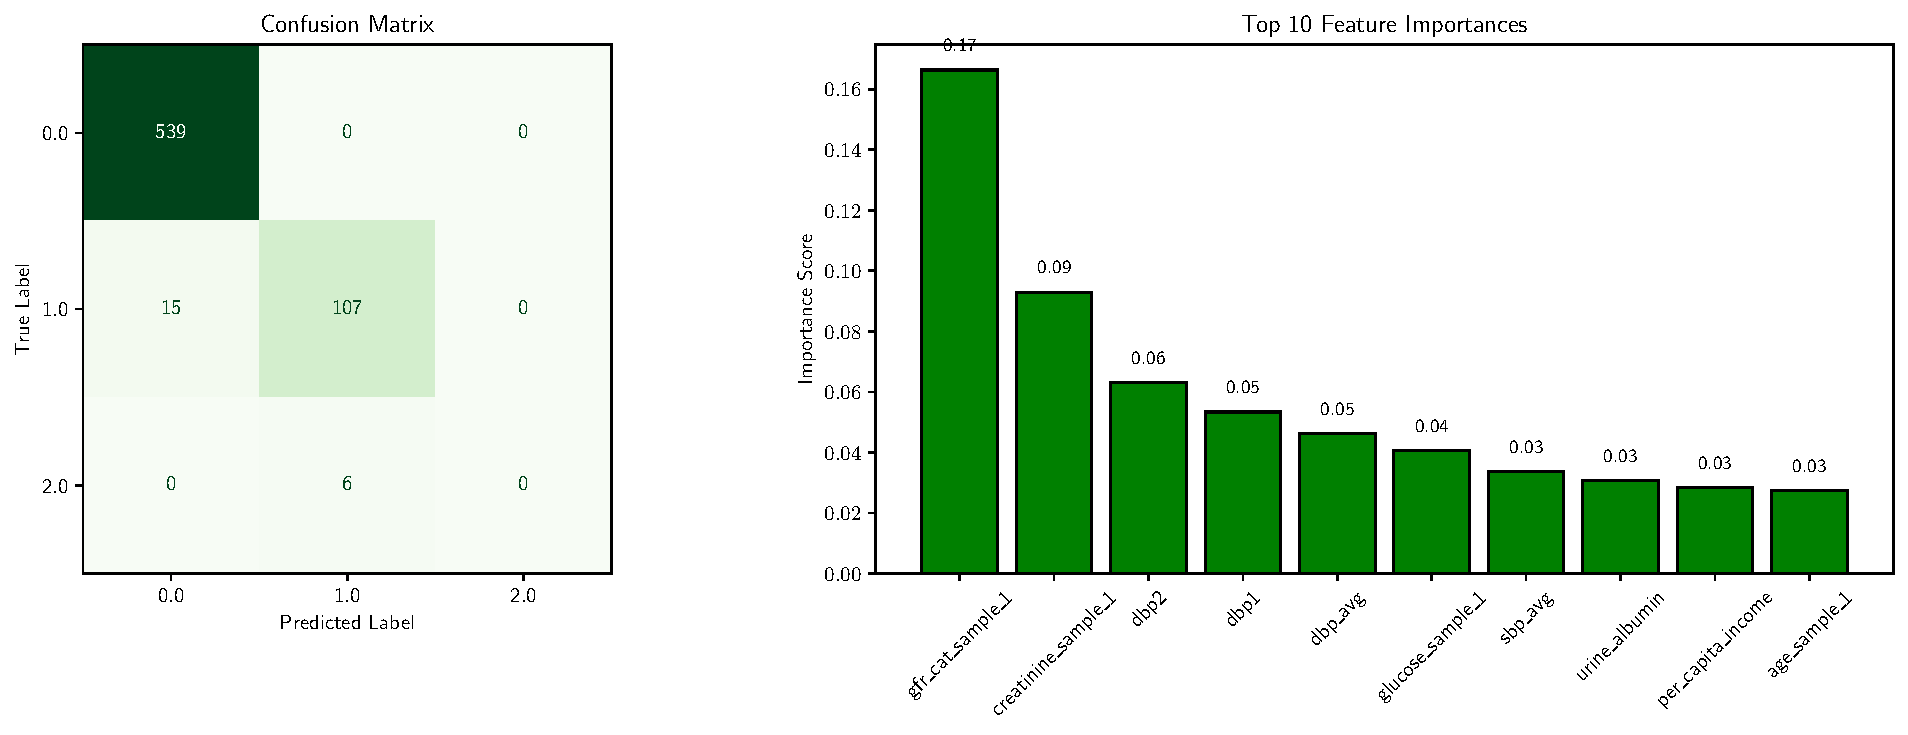
\includegraphics[scale=.35]{RF_summary.pdf}
    \end{figure}
\end{frame}

\begin{frame}{Number of Trees}
        \begin{figure}
        \centering
        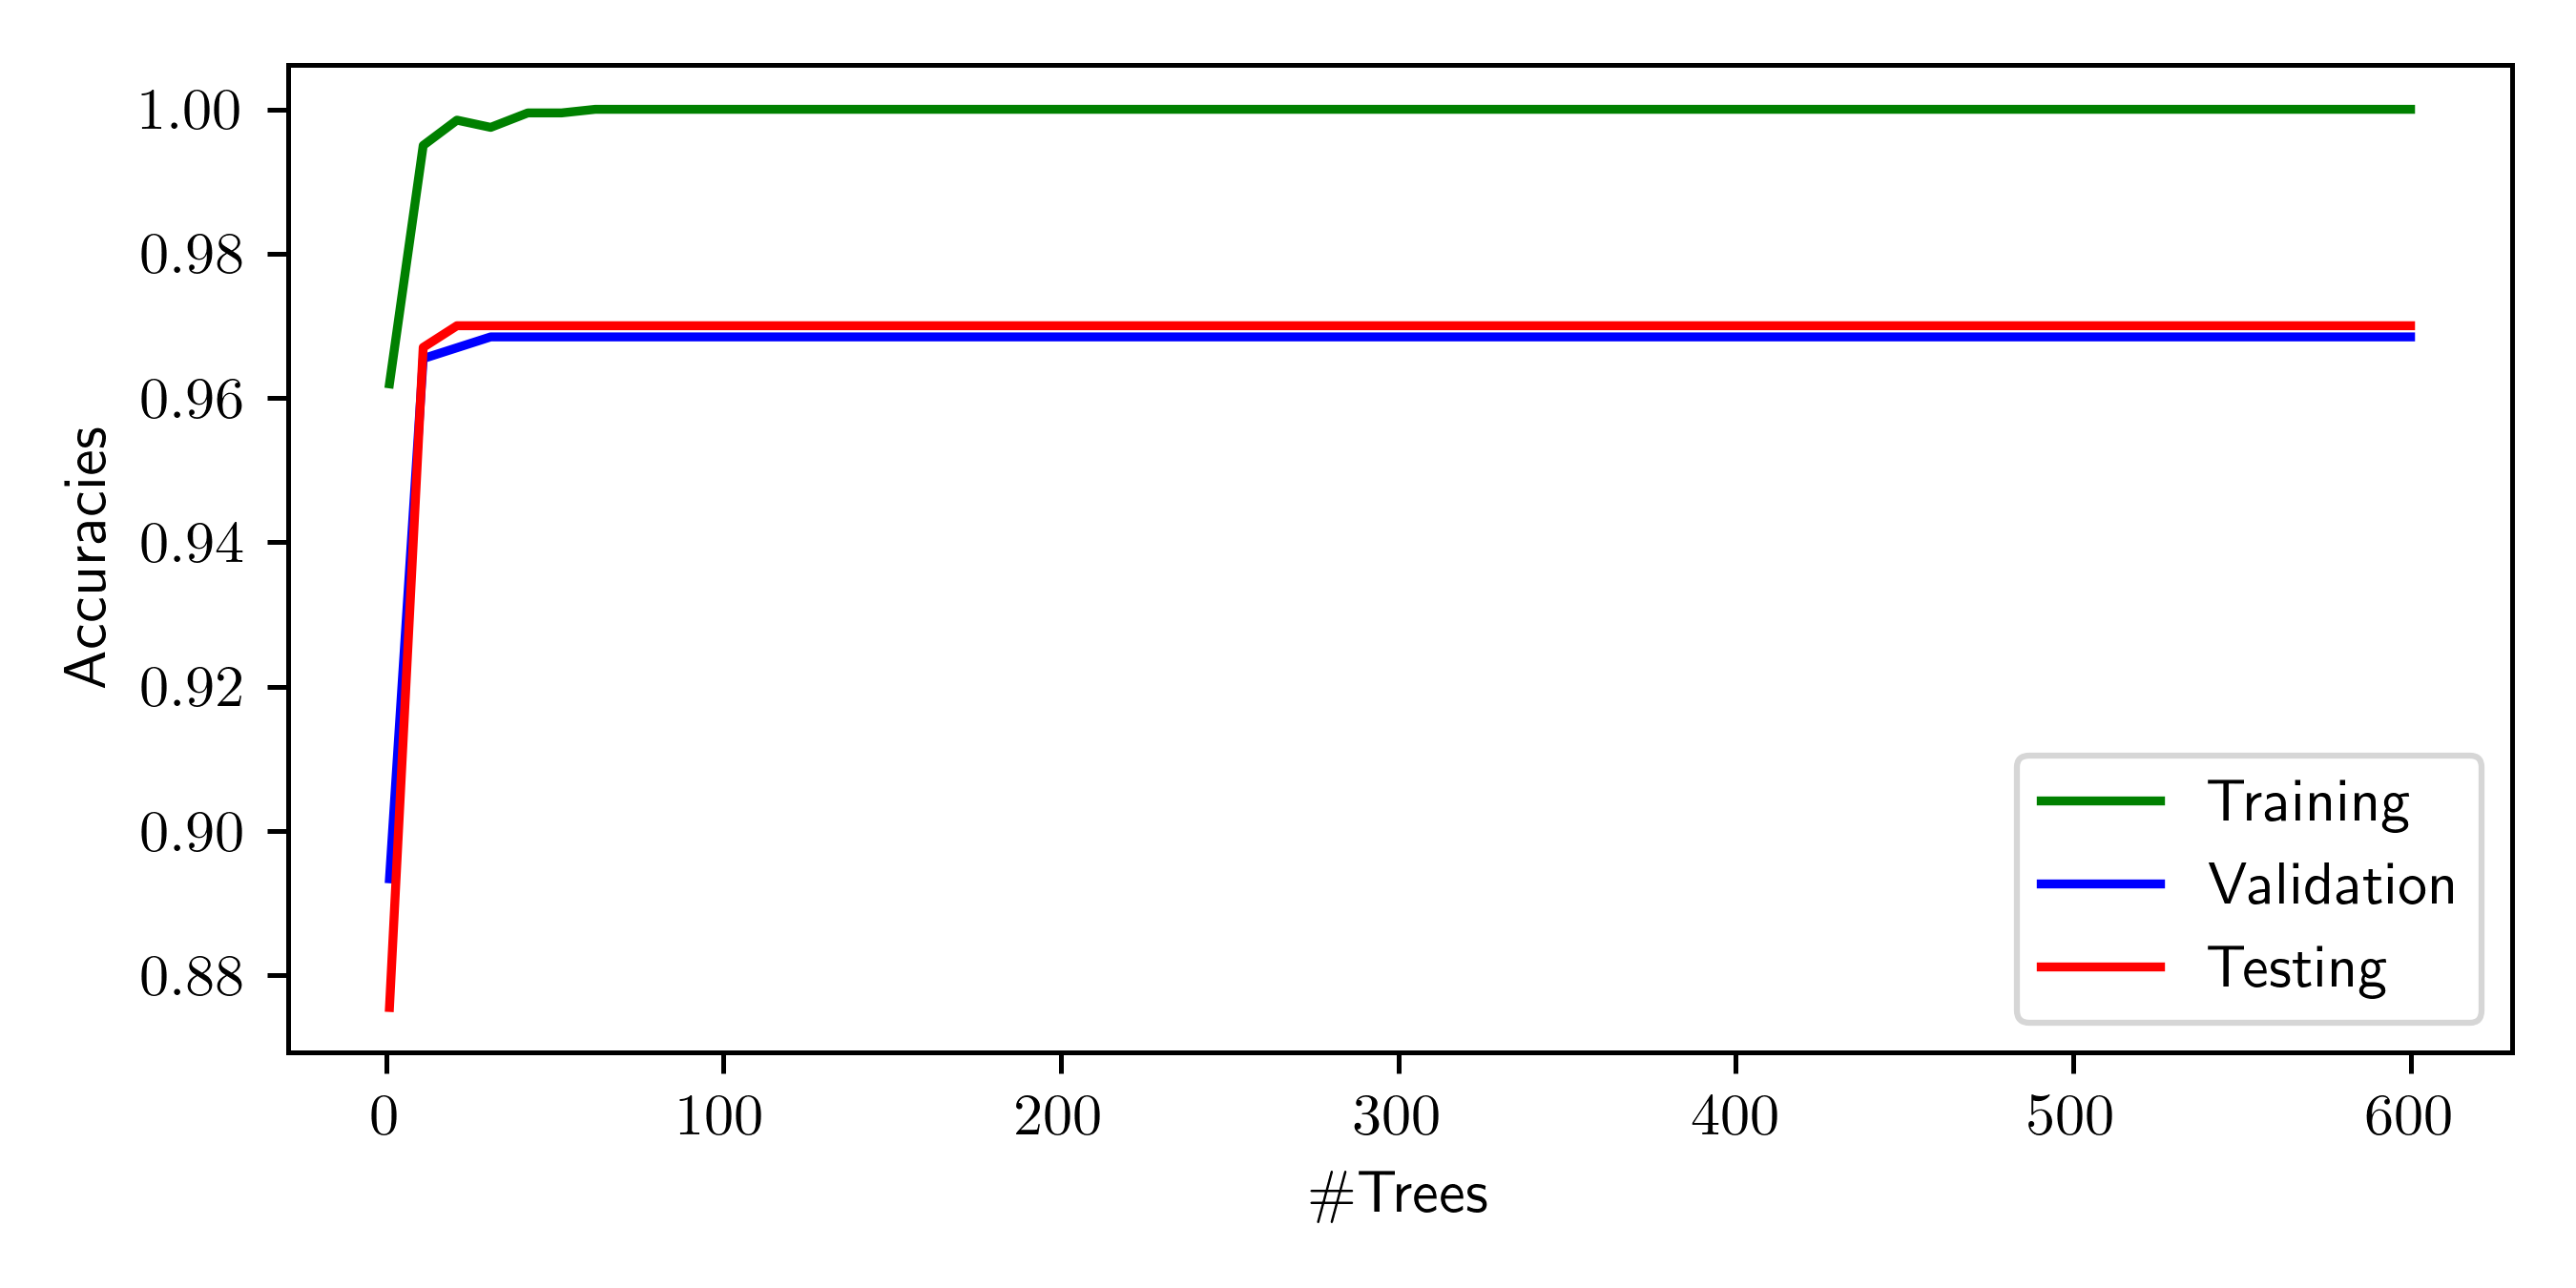
\includegraphics[scale=.5]{RF_acc_tree.png}
    \end{figure}
\end{frame}

\end{document}